% ===== Section 2: "Where are your trousers, professor?" (~18 min), then the break =====
\topicopener{jeans}{Պրոֆեսորի տաբատը}{Պրոֆեսո՛ր, տաբատդ ո՞ւր է}{Ինչպես են խելացի մարդիկ հիմարություններ անում}{panic}

% The absent-minded professor stereotype
\begin{frame}{Ցրված պրոֆեսորը}
  \begin{columns}[T]
    \begin{column}{0.56\textwidth}
      \begin{bookquote}
        Սպիտակ մազերով, սպիտակ խալաթով տղամարդ (գրեթե միշտ՝ տղամարդ), որ նկարագրում է պտղաճանճի գենոմը՝ միաժամանակ \textbf{կարագ քսելով փողկապին}։
      \end{bookquote}
      \onslide<3->{%
      \begin{card}[colback=peach!40!cardwhite]
        Խելքը ուժի նման չէ. ուժեղը ուժեղ է ամենուր, իսկ մի տեղ փայլուն մարդը մյուս տեղում կարող է անճար թվալ։
      \end{card}}
    \end{column}
    \begin{column}{0.38\textwidth}
      \centering
      \bigemoji[1.3cm]{scientist}\ \bigemoji[1.0cm]{boss}\ \bigemoji[0.9cm]{bread}\par\medskip
      \onslide<2->{%
      \begin{poll}
        Բարձրացրու ձեռքդ, եթե ճանաչում ես մեկին, ով մի բանում հանճար է, իսկ առօրյայում՝ անօգնական։
      \end{poll}}
    \end{column}
  \end{columns}
\end{frame}

% Factor analysis, with Burnett's headmaster example
\begin{frame}{Գործոնային վերլուծություն}
  \begin{columns}[c]
    \begin{column}{0.42\textwidth}
      Մեկ ընդհանուր խելք, թե՞ մի քանի տեսակ։ Վեճը շարունակվում է, ու պատասխանը, հավանաբար, երկուսի \textbf{համադրությունն} է։\par\medskip
      Կարևոր գործիքը՝ \textbf{գործոնային վերլուծությունը} (factor analysis). մեծ տվյալներից մաթեմատիկորեն «դուրս է քաշում» թաքնված գործոններ, որոնք նախապես հայտնի չեն։
    \end{column}
    \begin{column}{0.54\textwidth}
      \centering
      {\blackfont\small Դպրոցի գնահատականները «միջակ» են. ինչու՞}\par\smallskip
      \onslide<2->{% The book's headmaster example for factor analysis: middling marks overall, but split by subject
% maths did well and history badly. Made-up numbers (labelled as such on the slide).
% Horizontal bars so the subject names fit; ytick lists every coord (ytick=data would only take the first plot's).
\begin{tikzpicture}
  \begin{axis}[
      width=6.4cm, height=4.2cm,
      xbar, bar width=0.5cm, bar shift=0pt,
      xmin=0, xmax=100,
      symbolic y coords={hist, lit, phys, math},
      ytick={hist, lit, phys, math},
      yticklabels={Պատմություն, Գրականություն, Ֆիզիկա, Մաթեմատիկա},
      yticklabel style={font=\small, text=plum},
      xtick=\empty, axis x line=none,
      axis y line*=left, axis line style={plum},
      nodes near coords, nodes near coords style={font=\blackfont\small, text=plum},
      enlarge y limits=0.18, clip=false,
    ]
    \addplot[fill=amBlue, draw=none] coordinates {(81,math)};
    \addplot[fill=amBlue, draw=none] coordinates {(74,phys)};
    \addplot[fill=amBlue, draw=none] coordinates {(60,lit)};
    \addplot[fill=amRed, draw=none] coordinates {(33,hist)};
    \draw[plum, dashed, line width=0.8pt] ([yshift=-0.45cm]axis cs:62,hist) -- ([yshift=0.4cm]axis cs:62,math)
      node[anchor=south, font=\scriptsize, text=plum, inner sep=1pt] {միջինը՝ 62};
  \end{axis}
\end{tikzpicture}
\par}
      \onslide<3->{%
      \begin{tikzpicture}
        \node[say, font=\handfont\small] {Պատմության ուսուցիչնե՛ր...};
      \end{tikzpicture}\par
      {\scriptsize\color{plum!70!cream} թեև պատճառները կարող են շատ լինել · թվերը հորինված են\par}}
    \end{column}
  \end{columns}
\end{frame}

% Spearman's g
\begin{frame}{Սպիրմենի g-ն}
  \begin{columns}[c]
    \begin{column}{0.32\textwidth}
      Չարլզ Սպիրմենը գտավ, որ շատ տարբեր թեստերի արդյունքների հետևում կա \textbf{մեկ ընդհանուր գործոն}՝ g (general factor)։\par\medskip
      \onslide<2->{%
      \begin{card}[colback=butter!45!cream]
        Եթե գիտության մեջ մի բան կա, որ նման է առօրյա «խելք» բառին, դա g-ն է։
      \end{card}}
    \end{column}
    \begin{column}{0.64\textwidth}
      \centering
      % Spearman's g: one general factor behind performance on very different tests.
\begin{tikzpicture}[
    gtest/.style={draw=plum, line width=0.8pt, fill=cardwhite, rounded corners=2mm, align=center,
      font=\small, text=plum, inner sep=3pt, text width=3.0cm},
    garrow/.style={-{Stealth[length=2.4mm]}, plum, line width=1.1pt},
  ]
  \node[circle, draw=plum, line width=1.2pt, fill=butter, minimum size=1.5cm, font=\blackfont\fontsize{26}{28}\selectfont, text=plum] (g) at (0,0) {g};
  \node[gtest] (t1) at (-3.1,1.15) {\emoji{books}\ բառապաշար};
  \node[gtest] (t2) at (0,1.85) {\emoji{abacus}\ թվաբանություն};
  \node[gtest] (t3) at (3.1,1.15) {\emoji{puzzle}\ տրամաբանական խնդիրներ};
  \node[gtest] (t4) at (-3.1,-1.15) {\emoji{thought}\ հիշողություն};
  \node[gtest] (t5) at (0,-1.85) {\emoji{hourglass}\ արագություն};
  \node[gtest] (t6) at (3.1,-1.15) {\emoji{chess}\ տարածական պատկերացում};
  \foreach \t in {t1,t2,t3,t4,t5,t6}{\draw[garrow] (g) -- (\t);}
\end{tikzpicture}

    \end{column}
  \end{columns}
  \source{Spearman, Am. J. Psychol., 1904 (գրքում՝ «1920-ականներին»)}
\end{frame}

% g as the foundations of a house
\begin{frame}{g-ն տան հիմքն է}
  \begin{columns}[c]
    \begin{column}{0.4\textwidth}
      \centering
      \begin{tikzpicture}
        \fill[butter, draw=plum, line width=1pt] (-2.1,-0.45) rectangle (2.1,0);
        \node[font=\blackfont\normalsize, text=plum] at (0,-0.23) {g};
        \filldraw[fill=cardwhite, draw=plum, line width=1pt] (-1.8,0) rectangle (1.8,2.2);
        \filldraw[fill=brainpink!45!cardwhite, draw=plum, line width=1pt] (-2.1,2.2) -- (0,3.4) -- (2.1,2.2) -- cycle;
        \draw[plum, line width=0.6pt] (0,0) -- (0,2.2) (-1.8,1.1) -- (1.8,1.1);
        \node[visible on=<2->] at (-0.9,0.5) {\showon{2-}{\bigemoji[0.6cm]{books}}};
        \node[visible on=<2->] at (0.9,0.5) {\showon{2-}{\bigemoji[0.6cm]{puzzle}}};
        \node[visible on=<2->] at (-0.9,1.6) {\showon{2-}{\bigemoji[0.6cm]{abacus}}};
        \node[visible on=<2->] at (0.9,1.6) {\showon{2-}{\bigemoji[0.6cm]{musical}}};
      \end{tikzpicture}
    \end{column}
    \begin{column}{0.56\textwidth}
      g-ն ամբողջ խելքը չէ, այլ նրա \textbf{միջուկը}՝ ինչպես տան հիմքն ու կմախքը։\par\medskip
      \onslide<2->{Կահույք ու նոր սենյակներ կարող ես ավելացնել, բայց եթե հիմքը թույլ է, իմաստ չունի։\par\medskip}
      \onslide<3->{%
      \begin{bookquote}
        Կարող ես սովորել բոլոր խրթին բառերն ու հիշողության հնարքները, բայց առանց ամուր g-ի դրանցով շատ բան չես անի։
      \end{bookquote}}
    \end{column}
  \end{columns}
\end{frame}

% g and working memory, the prefrontal cortex
\begin{frame}{g-ն ու աշխատանքային հիշողությունը}
  \begin{columns}[c]
    \begin{column}{0.52\textwidth}
      \begin{itemize}
        \item \textbf{Աշխատանքային հիշողություն} (working memory)՝ կարճաժամկետ հիշողության տեղեկությունը մշակելը, «օգտագործելը»
        \item<2-> 2000-ականներ, Կլաուս Օբերաուերի խումբը. ով լավ է աշխատանքային հիշողության թեստերում, լավ է նաև IQ թեստերում
        \item<3-> Երկուսն էլ կախված են \textbf{նախաճակատային կեղևից} (prefrontal cortex)
      \end{itemize}
    \end{column}
    \begin{column}{0.44\textwidth}
      \centering
      \onslide<3->{%
      \begin{tikzpicture}[scale=0.85]
        \brainbg
        \brainfill{pfc}{amRed!45!cream}
        \brainlines
        \node[font=\small, text=plum, align=center, anchor=south] at (0.9,3.75) {նախաճակատային\\ կեղև};
        \draw[plum, line width=0.7pt] (0.9,3.75) -- (0.9,2.8);
        \node[font=\scriptsize, text=plum!70!cream] at (2.9,-0.6) {ճակատը՝ ձախ կողմում};
      \end{tikzpicture}}
    \end{column}
  \end{columns}
  \source{Süß et al., Intelligence, 2002}
\end{frame}

% Fluid and crystallised intelligence
\begin{frame}{Հեղուկ և բյուրեղացած ինտելեկտ}
  \relax{\small Աշխատանքային հիշողությունը հիմնականում բառերով է աշխատում, իսկ խելքը՝ ամեն տեսակ տեղեկության հետ։ 1940-60-ականներին Ռայմոնդ Քեթելն ու Ջոն Հորնը առանձնացրին երկու տեսակ.}\par
  \begin{columns}[T]
    \begin{column}{0.47\textwidth}
      \begin{card}[colback=amBlue!12!cardwhite]
        \emoji[1.3em]{puzzle}\ {\blackfont Հեղուկ} (fluid intelligence)\par\smallskip
        \textbf{Նոր} տեղեկության հետ աշխատելու, այն կիրառելու ունակությունը\par\smallskip
        {\small Ռուբիկի խորանարդ, կամ հասկանալ, թե ինչու զուգընկերդ քեզ հետ չի խոսում, երբ ոչինչ չես հիշում}
      \end{card}
    \end{column}
    \begin{column}{0.47\textwidth}
      \onslide<2->{%
      \begin{card}[colback=amOrange!15!cardwhite]
        \emoji[1.3em]{books}\ {\blackfont Բյուրեղացած} (crystallized intelligence)\par\smallskip
        Հիշողության մեջ \textbf{կուտակված} գիտելիքը\par\smallskip
        {\small 1950-ականների անհայտ ֆիլմի դերասանը վիկտորինայում, մայրաքաղաքները, օտար լեզուն}
      \end{card}}
    \end{column}
  \end{columns}
\end{frame}

% Chat quiz: fluid or crystallised?
\begin{frame}{Հեղուկ, թե՞ բյուրեղացած}
  \begin{columns}[c]
    \begin{column}{0.6\textwidth}
      \begin{enumerate}
        \item Լուծել սուդոկու, որ առաջին անգամ ես տեսնում \onslide<3->{\ \chip[amBlue!20!cardwhite]{}{Հ}}
        \item Հիշել Ավստրալիայի մայրաքաղաքը \onslide<3->{\ \chip[amOrange!25!cardwhite]{}{Բ}}
        \item Հասկանալ նոր սեղանի խաղի կանոններն ու հաղթել \onslide<3->{\ \chip[amBlue!20!cardwhite]{}{Հ}}
        \item Անգլերեն տեքստ թարգմանել \onslide<3->{\ \chip[amOrange!25!cardwhite]{}{Բ}}
        \item Լուծել քննական խնդիր, որի նմանը չես տեսել \onslide<3->{\ \chip[amBlue!20!cardwhite]{}{Հ}}
      \end{enumerate}
    \end{column}
    \begin{column}{0.36\textwidth}
      \begin{chatbox}
        Գրիր հինգ տառ, օրինակ՝ \textbf{ՀԲՀԲԲ}\par\smallskip
        Հ՝ հեղուկ, Բ՝ բյուրեղացած
      \end{chatbox}
      \onslide<2->{\centering\mascot[1.8cm]{thinking}\par}
    \end{column}
  \end{columns}
\end{frame}

% Fluid declines with age, crystallised stays
\begin{frame}{Տարիքի հետ}
  \begin{columns}[c]
    \begin{column}{0.5\textwidth}
      \centering
      % Schematic only (no data): fluid intelligence falls with age, crystallised stays roughly stable (the book's claim).
\begin{tikzpicture}
  \begin{axis}[
      width=6.8cm, height=4.6cm,
      xmin=18, xmax=85, ymin=0, ymax=1.05,
      xtick={20,30,40,50,60,70,80}, ytick=\empty,
      xlabel={տարիք}, ylabel={արդյունք},
      label style={font=\small, text=plum}, tick label style={font=\small, text=plum},
      axis lines=left, axis line style={plum, -{Stealth}},
      clip=false,
    ]
    \addplot[amBlue, line width=2pt, smooth, tension=0.6] coordinates
      {(20,0.86) (27,0.88) (35,0.81) (45,0.71) (55,0.6) (65,0.48) (75,0.37) (82,0.31)};
    \addplot[amOrange, line width=2pt, smooth, tension=0.6] coordinates
      {(20,0.55) (30,0.67) (40,0.75) (50,0.79) (60,0.8) (70,0.79) (82,0.76)};
    \node[anchor=south, font=\blackfont\small, text=amOrange!80!black] at (axis cs:62,0.83) {բյուրեղացած};
    \node[anchor=north east, font=\blackfont\small, text=amBlue] at (axis cs:52,0.6) {հեղուկ};
    \node[anchor=south west, font=\scriptsize, text=plum!60!cream] at (axis cs:19,0.02) {սխեմատիկ};
  \end{axis}
\end{tikzpicture}

    \end{column}
    \begin{column}{0.46\textwidth}
      \begin{itemize}
        \item \textbf{Հեղուկը նվազում է}. 80-ում թեստն ավելի վատ ես գրում, քան 30-ում
        \item<2-> Նախաճակատային կեղևը շատ է աշխատում, ու դրա թափոնները (ազատ ռադիկալներ) տարիքի հետ «մաշում» են այն
        \item<3-> \textbf{Բյուրեղացածը կայուն է}. 18-ում սովորած ֆրանսերենը 85-ում էլ կիմանաս, եթե 19-ում չես մոռացել
      \end{itemize}
    \end{column}
  \end{columns}
\end{frame}

% Where in the brain
\begin{frame}{Ուղեղում՝ տարբեր տեղեր}
  \begin{columns}[c]
    \begin{column}{0.46\textwidth}
      \begin{card}[colback=amBlue!12!cardwhite]
        {\blackfont Հեղուկ}. անծանոթ նախշեր, «ավելորդը գտիր» խնդիրներ\par
        $\rightarrow$ \textbf{նախաճակատային կեղև}
      \end{card}
      \onslide<2->{%
      \begin{card}[colback=amOrange!15!cardwhite]
        {\blackfont Բյուրեղացած}. բառացանկեր, վիկտորինաներ\par
        $\rightarrow$ \textbf{ավելի լայն կեղև}, օր.՝ գագաթային բիլթը և Բրոկայի գոտին (խոսք)
      \end{card}}
    \end{column}
    \begin{column}{0.5\textwidth}
      \centering
      \begin{tikzpicture}[scale=0.9]
        \brainbg
        \brainfill{pfc}{amBlue!40!cream}
        \brainfill{parietal}{amOrange!35!cream}
        \brainlines
        \fill[amOrange!80!cream, draw=plum, line width=0.6pt, visible on=<2->] (1.85,1.75) circle (0.24);
        \fill[amOrange!80!cream, draw=plum, line width=0.6pt, visible on=<2->] (3.85,2.2) circle (0.26);
        \node[font=\scriptsize, text=plum, align=center, anchor=south] at (0.8,3.7) {նախաճակատային\\ կեղև};
        \node[font=\scriptsize, text=plum, align=center, anchor=south, visible on=<2->] at (4.4,3.55) {գագաթային\\ բիլթ};
        \node[font=\scriptsize, text=plum, align=center, anchor=north, visible on=<2->] (br) at (1.4,0.2) {Բրոկայի\\ գոտի};
        \draw[plum, line width=0.6pt, visible on=<2->] (br.north) -- (1.8,1.55);
      \end{tikzpicture}
    \end{column}
  \end{columns}
\end{frame}

% Miles Kington's tomato
\begin{frame}{Լոլիկն ու մրգային աղցանը}
  \begin{center}
    \begin{tikzpicture}
      \node[draw=plum, line width=0.9pt, fill=cardwhite, rounded corners=4mm, inner xsep=7mm, inner ysep=4mm,
            text width=10.4cm, align=center, font=\blackfont\large, text=plum] (q)
        {«Գիտելիքը իմանալն է, որ լոլիկը միրգ է։ Իմաստությունը այն մրգային աղցանի մեջ չդնելն է»};
      \begin{scope}[on background layer]
        \fill[plum, rounded corners=4mm] ([xshift=1.2mm, yshift=-1.2mm]q.south west) rectangle ([xshift=1.2mm, yshift=-1.2mm]q.north east);
      \end{scope}
      \node[anchor=north east, font=\small, text=plum!80!cream] at ([yshift=-2mm]q.south east) {Մայլս Քինգթոն, բրիտանացի լրագրող};
      \node at ([xshift=2mm, yshift=-1mm]q.north west) {\tomato[1.3]};
    \end{tikzpicture}
  \end{center}
  \begin{columns}[T]
    \begin{column}{0.47\textwidth}
      \onslide<2->{\chip[amOrange!25!cardwhite]{books}{Բյուրեղացած}\ գիտես, որ լոլիկը միրգ է\par}
    \end{column}
    \begin{column}{0.47\textwidth}
      \onslide<3->{\chip[amBlue!20!cardwhite]{puzzle}{Հեղուկ}\ կիրառում ես. աղցանը չես փչացնում\par}
    \end{column}
  \end{columns}
  \vspace{2mm}
  \onslide<4->{\centering Հեղուկ ինտելեկտը շատ նման է \textbf{ողջախոհությանը} (common sense)։\par}
\end{frame}

% Footballers and savants
\begin{frame}{Ֆուտբոլիստներն ու սավանտները}
  \begin{columns}[c]
    \begin{column}{0.58\textwidth}
      Որոշ գիտնականների համար երկու տեսակն էլ քիչ է։\par\medskip
      \begin{itemize}
        \item<2-> \textbf{Ֆուտբոլիստները} հաճախ դպրոցում չեն փայլել, բայց խաղը պահանջում է ճշգրիտ վերահսկում, ուժի ու անկյունների հաշվարկ, ամբողջ դաշտի պատկերացում, ու երկրպագուների գոռոցն անտեսելու կամք
        \item<3-> \textbf{Սավանտներ} (savants)՝ նյարդաբանական խանգարում ունեցող մարդիկ, որոնք զարմանալի ունակություններ ունեն մաթեմատիկայում, երաժշտության կամ հիշողության մեջ
      \end{itemize}
    \end{column}
    \begin{column}{0.38\textwidth}
      \centering
      \onslide<4->{%
      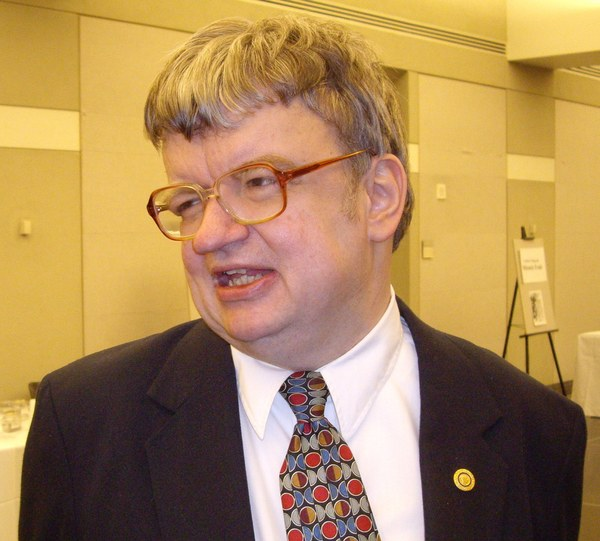
\includegraphics[width=0.8\linewidth]{kim_peek.jpg}\par\smallskip
      {\small \textbf{Քիմ Փիք}՝ «Անձրևի մարդը» ֆիլմի հերոսի նախատիպը. բառացի հիշում էր մինչև \textbf{12 000 գիրք}\par}}
    \end{column}
  \end{columns}
\end{frame}

% Thurstone's seven primary mental abilities, told as a cage fight
\begin{frame}{Թերսթոնի 7 «առաջնային» ունակությունը (1938)}
  \begin{columns}[T]
    \begin{column}{0.49\textwidth}
      \small
      \begin{enumerate}
        \item<2-> \textbf{Բառերի ըմբռնում}. «Հե՜յ, ես գիտեմ՝ դա ինչ է նշանակում»
        \item<3-> \textbf{Խոսքի սահունություն}. «Արի երեսիս ասա, ինտելեկտուալ առումով սակավաշնորհ արարած»
        \item<4-> \textbf{Հիշողություն}. «Սպասիր, ես քեզ ճանաչում եմ. դու MMA-ի աշխարհի չեմպիոնն ես»
        \item<5-> \textbf{Թվաբանություն}. «Իմ հաղթելու շանսը 1 է 82 523-ից»
      \end{enumerate}
    \end{column}
    \begin{column}{0.49\textwidth}
      \small
      \begin{enumerate}\setcounter{enumi}{4}
        \item<6-> \textbf{Ընկալման արագություն}. «Նրա վզնոցը մարդկային ատամների՞ց է»
        \item<7-> \textbf{Ինդուկտիվ դատողություն}. «Նրան հանգստացնելու ամեն փորձ ավելի կկատաղեցնի»
        \item<8-> \textbf{Տարածական պատկերացում}. «Եթե սեղանը շրջեմ, կդանդաղի, ու կհասցնեմ պատուհանից թռչել»
      \end{enumerate}
      \vspace{1mm}
      \onslide<9->{%
      \begin{card}[colback=lavender!35!cardwhite]
        Ավելի սովորական վերլուծությամբ նրա տվյալներում... \textbf{նորից g-ն գտան}։
      \end{card}}
    \end{column}
  \end{columns}
\end{frame}

% Thurstone found g again; Gardner's multiple intelligences
\begin{frame}{Գարդների բազմակի ինտելեկտները}
  \begin{columns}[T]
    \begin{column}{0.47\textwidth}
      \begin{card}[colback=mint!35!cardwhite]
        {\blackfont 1980-ականներ. Հովարդ Գարդներ}\par\smallskip
        Ուղեղի վնասվածքով պացիենտների մոտ որոշ ունակություններ պահպանվում էին։ Ուրեմն խելքի \textbf{մի քանի տեսակ} կա։\par
        Կան նաև \textbf{երաժշտական} ու \textbf{անձնային} ինտելեկտներ՝ շփվել մարդկանց հետ, հասկանալ ինքդ քեզ։
      \end{card}
    \end{column}
    \begin{column}{0.47\textwidth}
      \onslide<2->{%
      Բազմակի ինտելեկտների տեսությունը (multiple intelligences) սիրված է. \textbf{բոլորը կարող են խելացի լինել}։ Բայց այդ դեպքում բառը կորցնում է գիտական իմաստը։\par\medskip}
      \onslide<3->{%
      \begin{bookquote}
        Ինչպես մարզական օրը բոլորին մեդալ տալը՝ միայն գալու համար։ Հաճելի է, բայց սպորտի իմաստը կորչում է։ \emoji{medal}
      \end{bookquote}}
    \end{column}
  \end{columns}
\end{frame}

% g plus preferences; swimmers and tennis players; phrenology as the old opposite view
\begin{frame}{Լողորդներն ու թենիսիստները}
  \begin{columns}[c]
    \begin{column}{0.6\textwidth}
      \begin{itemize}
        \item Տվյալները մեծ մասամբ խոսում են \textbf{g-ի ու անձնական նախասիրությունների} օգտին
        \item<2-> Երաժշտության ու մաթեմատիկայի մեջ փայլողները նույն g-ն են կիրառում տարբեր խնդիրներում
        \item<3-> Լողորդն ու թենիսիստը նույն մկաններն են օգտագործում, «թենիսի մկաններ» չկան։ Բայց լողի չեմպիոնը ինքնաբերաբար թենիսի չեմպիոն չի դառնա
      \end{itemize}
    \end{column}
    \begin{column}{0.36\textwidth}
      \centering
      \onslide<4->{%
      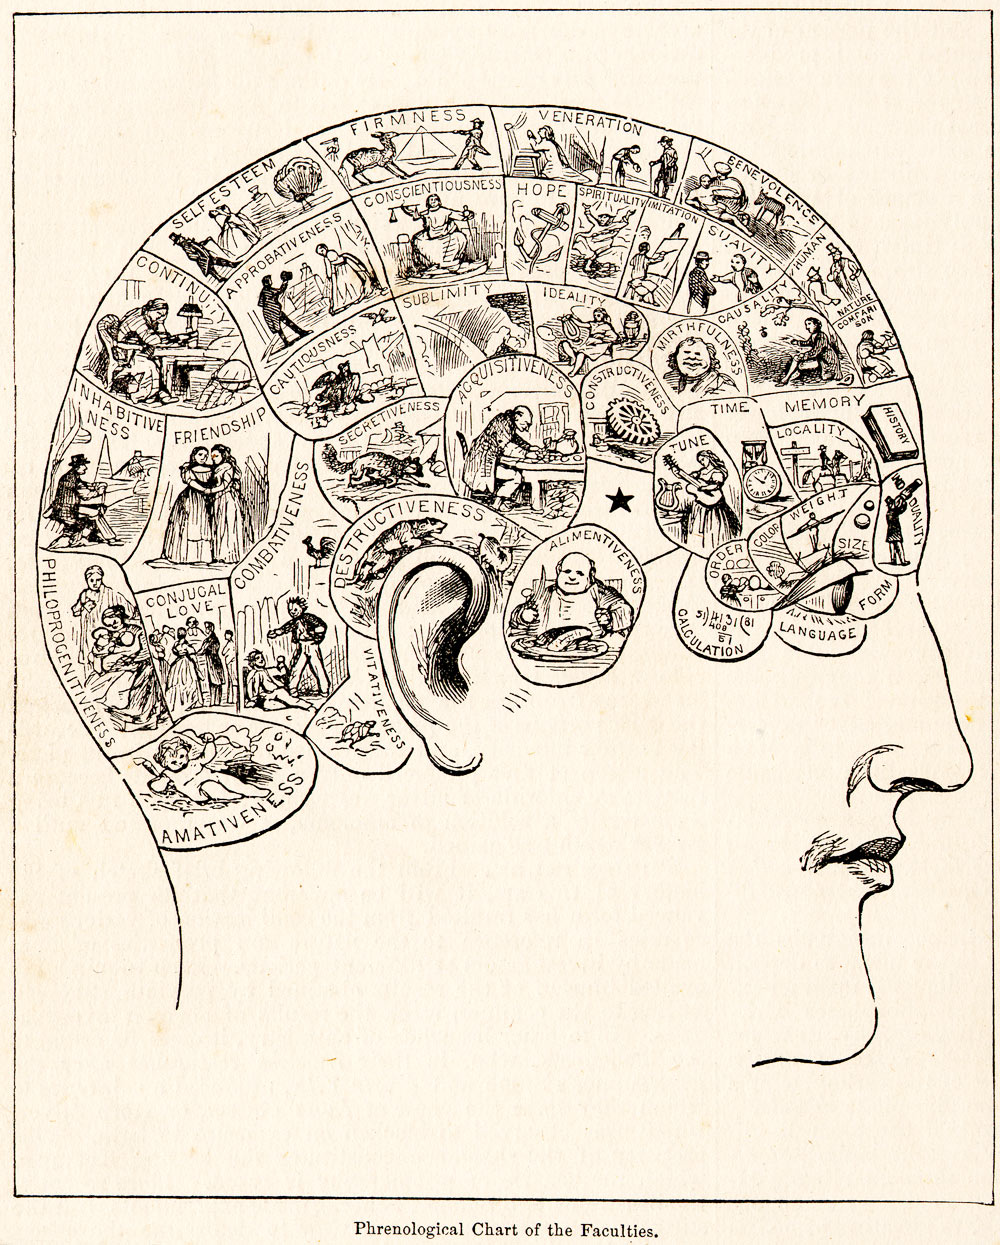
\includegraphics[width=0.5\linewidth]{phrenology_chart.jpg}\par\smallskip
      {\scriptsize 19-րդ դարի ֆրենոլոգիա. ամեն ունակություն՝ գանգի իր «թմբիկում»\par}\smallskip
      {\small Այսօր. խելքը ուղեղի մասերի \textbf{համագործակցությունն} է, ոչ թե առանձին «սենյակներ»։\par}}
    \end{column}
  \end{columns}
\end{frame}

% So why does the professor forget his trousers?
\begin{frame}{Ուրեմն ինչու՞ է պրոֆեսորը մոռանում տաբատը}
  \begin{columns}[c]
    \begin{column}{0.56\textwidth}
      \begin{itemize}
        \item Բոլորս մեր խելքն ուղղում ենք որոշակի կողմեր՝ նախասիրության, դաստիարակության, միջավայրի կամ ուղեղի նուրբ առանձնահատկությունների պատճառով
        \item<2-> Խելացի մարդը հիմարություն է անում ոչ թե որովհետև խելքը չի հերիքում, այլ որովհետև \textbf{մտքով ուրիշ տեղ է}
      \end{itemize}
    \end{column}
    \begin{column}{0.38\textwidth}
      \centering
      \onslide<3->{%
      \mascot[2.0cm]{smug}\par\smallskip
      \begin{bookquote}
        Լավ կողմն այն է, որ նրանց վրա կարելի է ծիծաղել. միևնույն է, չեն նկատի։
      \end{bookquote}}
    \end{column}
  \end{columns}
\end{frame}

% ---------------------------------------------------------------- break
\notopic
\begin{frame}[plain]
  \begin{tikzpicture}[remember picture, overlay]
    \fill[butter!60!cream] (current page.south west) rectangle (current page.north east);
    \node at ([yshift=8mm]current page.center) {\mascot[4cm]{sleepy}};
    \node[anchor=north, font=\titlefont\fontsize{30}{32}\selectfont, text=plum] at ([yshift=-17mm]current page.center) {Ընդմիջում};
    \node[anchor=north, font=\mediumfont\large, text=plum] at ([yshift=-31mm]current page.center)
      {5 րոպե \emoji{coffee}\quad Կանգնիր, ձգվիր, ջուր խմիր};
  \end{tikzpicture}
\end{frame}
